\section{The ATLAS Experiment}
ATLAS (A Toroidal LHC ApparatuS) is one of two general purpose detectors at CERN (the European Organization for Nuclear Research) near Geneva in Switzerland. These detectors collect data from the collisions provided by the worlds highest energy particle accelerator~\cite{lhc-design-report}, the Large Hadron Collider (LHC) situated at CERN. \\

In this section, information about the LHC and the ATLAS detector are given. This includes technical aspects of the ATLAS detector and the processing of data into meaningful physics objects to be used in analyses.

\subsection{Large Hadron Collider (LHC)}
The LHC is a circular 27km particle accelerator located in an underground tunnel on the border between France and Switzerland. The accelerator consists of supercooled, superconducting magnets which accelerate and collide beams of protons at centre-of-mass energies up to $\sqrt{s} = 13$TeV at instantaneous luminosities of $\mathcal{L} \sim 10^{34}$cm$^{-2}$s$^{-1}$. The LHC mainly produces these $pp$ collisions, however heavy-ion collisions can be produced (typically lasting a month, annually) which reach centre-of-mass energies of $\sqrt{s} = 5.02$TeV$/$nucleon at instantaneous luminosities of $\mathcal{L} \sim 10^{27}$cm$^{-2}$s$^{-1}$. $pp$ beams consist of bunches of protons which collide every 25ns, corresponding to a frequency of 40MHz. \\ 

Several accelerator systems are used to accelerate protons and heavy ions to such high energies. Protons are extracted from a tank of ionised hydrogen gas and are injected into the Linear Accelerator 2 (LINAC), where they are linearly accelerated to momenta of 50MeV. The proton bunches are then sequentially accelerated by a chain of circular accelerators. The chain starts with the Booster which accelerates the protons to momenta of up to 1.4GeV. The proton bunches are then fed through to the Proton Synchrotron (PS) and the Super Proton Synchrotron (SPS) which accelerate the protons to momenta of up to 25GeV and 450GeV respectively. The protons are then transferred to two beam pipes of the LHC where they travel in opposite directions. Both proton beams are accelerated to their final momenta of 6.5TeV, resulting in a centre-of-mass energy of 13TeV. These proton beams then collide at one of the four main interaction points situated along the LHC. \\

The four main experiments located at the interaction points are ATLAS, the Compact Muon Solenoid (CMS), Large Hadron Collider Beauty (LHCb) Experiment and A Large Ion Collider Experiment (ALICE). ATLAS and CMS are general-purpose detectors which investigate a wide range of physics processes. Since both ATLAS and CMS can measure the same processes, they are able to cross-check and validate measurements taken by one another. LHCb is specifically designed to study decays of particles containing $b$-quarks. ALICE is designed to study the strongly interacting quark-gluon plasma which is formed at extremely high energy densities.\\

At the interaction points, the two proton beams which consist of protons in closely packed bunches, travel in opposite directions to one another and collide. We are only able to study one $pp$ collision (event) at a time, however many hard $pp$ collisions can occur per bunch crossing. These additional collisions are referred to as \textit{pile-up}. Pileup complicates the reconstruction of the particles originating from the hard collision of interest. 



\section{The ATLAS Detector}
The ATLAS detector is a general purpose particle detector, located at one of the four interaction points along the LHC beam pipe (100 m below ground). In Figure~\ref{fig:atlas-detector}, the schematic of the ATLAS detector, is shown.


\begin{figure}[h!]
 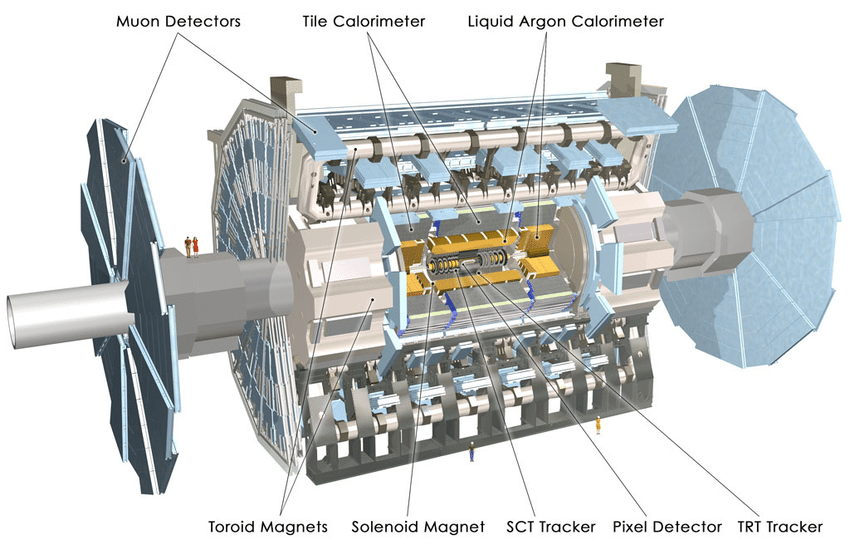
\includegraphics[width=0.5\textwidth]{figures/theoryFigs/atlasDetector.png}
 \centering
\caption{Schematic of the ATLAS detector~\cite{Collaboration_2008}}
\label{fig:atlas-detector}
\end{figure}


The detector is cylindrically shaped which covers close to 4$\pi$ in solid angle. It has a length of 44 m, a diameter of 25 m and a mass of 7000 tons. ATLAS consists of four main sub-detectors arranged in concentric cylindrical layers around the beam pipe. These include the inner detector, the electromagnetic calorimeter, the hadronic calorimeters and the muon spectrometer. The sub-detectors record the momenta, energies and trajectories of different particles produced in the collider, allowing for the reconstruction and identification of these particles to be used in physics analyses.

\subsection{Coordinate System and Kinematics}

The ATLAS detector adopts a right-handed coordinate system. The origin is at the nominal interaction point with the beam direction defining the $z-$axis. The $x-y$ plane (or transverse plane) is perpendicular to the beam line, with the $x-$axis pointing towards the centre of the LHC ring and the $y$-axis pointing upwards towards the Earth's surface. The azimuthal angle, $\phi \in [-\pi, \pi]$, is measured in the transverse plane with respect to the positive $x-$axis. The polar angle, $\theta \in [0,\pi]$, is measured in the $z-y$ plane with respect to the positive $y-$axis. A quantity called the pseudorapidity, $\eta \in [0,\infty]$ is defined as,

\begin{equation}
\eta = -\ln{\tan{\left(\frac{\theta}{2}\right)}}
\end{equation}
$\eta$ is often used as a measure of the polar angle, instead of $\theta$, since the difference in $\eta$ between two particles, $\Delta \eta$, is invariant under a Lorentz boost in the $z-$direction. The angular distance between two physics objects, $\Delta R$, can be written as,

\begin{equation}
\Delta R = \sqrt{(\Delta\phi)^{2} + (\Delta\eta)^{2}}
\end{equation}
where $\Delta\phi$ is the difference in $\phi$ between the two physics objects of interest. Quantities defined in the transverse plane are often used to describe the kinematics of physics objects in hadron collider experiments. The transverse momentum, $p_{T}$, is defined as,
\begin{equation}
p_{T}= \sqrt{(p_{x})^{2} + (p_{y})^{2}}
\end{equation}
where $p_{x}$ and $p_{y}$ are the $x$ and $y$ components of the physics object's momenta, respectively. The transverse energy, $E_{T}$, is defined as,
\begin{equation}
E_{T} = \sqrt{m^{2} + p_{T}^{2}}
\end{equation}
where $m$ is the invariant mass of the physics object. 

%The energy and momentum in particle collisions are conserved, however the absence of detector elements along the beam line, neutrinos escaping from the detector and unknown initial parton momenta restricts us from fully reconstructing the initial and final state particles. We can however, quantify the amount of transverse momenta which is - possibly go in particle ID section


\subsection{Inner Detector}
The inner detector is the first layer of concentric cylindrical sub-detector layers in the ATLAS detector. It is used to identify charged particles and reconstruct the trajectories of charged particles produced in the collisions via energy deposition in semiconductor material (hits) and the ionisation of gas. It consists of three complementary sub-detectors (in order from nearest to farthest from the beam pipe): the Pixel Detector, the Semiconductor Tracker (SCT) and the Transition Radiation Detector (TRT). The Pixel Detector and SCT are based on semiconductor technology and have the highest granularity of any sub-detector in ATLAS, in order to cope with the high frequency of collisions near the interaction point. The TRT consists of drift tubes (straws) containing a mixture of gas ($70\%$ Xe, $27\%$ CO$_{2}$ and $3\%$O$_{2}$), which allows measurement of the energy deposited by charged particles through the ionisation of the gas. Solenoid magnets surround the inner detector and bend the trajectories of charged particles. The charges and momenta of particles can be inferred from their bent trajectories, which are reconstructed by the hits produced via energy deposition in the Inner Detector.

\subsection{Electromagnetic and Hadronic Calorimeters}
The Electromagnetic Calorimeter (ECAL) and Hadronic Calorimeter (HCAL) surround the Inner Detector, with the ECAL nearer to the beam line. The ECAL and HCAL provide accurate measurements of the energy of particles which interact electromagnetically (e.g. photons and electrons) and hadronically (e.g. jets), respectively. Particles entering the calorimeters interact with the detector material and create either a electromagnetic shower (in the ECAL) or a hadronic shower (in the HCAL), depositing all their energy in the calorimeter cells. The calorimeters consist of an active material and a passive absorber material. Active materials are used to measure the energy deposited by the particles and passive absorber materials induce the electromagnetic and hadronic showers. The ECAL uses liquid argon (LAr) as its active material and lead as its absorber material. The HCAL uses alternating steel absorber layers and plastic scintillating tile layers as its active material. The primary mechanism of energy deposition in the ECAL is through bremsstrahlung (for electrons) and pair production (photons). Hadrons usually deposit a small amount of their energy in the ECAL, and interact via inelastic scattering with the nuclei of the detector material. The hadronic showers (jets) produced in these nuclear interactions travel much further than an electromagnetic shower, and for that reason, the volume of the is designed HCAL occupies a much larger space than that of the ECAL.

\subsection{Muon Spectrometer}
The Muon Spectrometer (MS) is the outermost sub-detector of ATLAS and surrounds the HCAL. Muons traverse through the inner detector and calorimeters, with minimal energy loss, before reaching the MS. The MS consists of trigger and high-precision tracking systems. Large superconducting toroid shaped magnets deflect the incoming muons to measure their trajectories and subsequently their momenta via the curvature of the trajectories. The MS measures muon trajectories as they ionize gas (filled with Ar and CO$_{2}$ gas) in the MS drift chambers.

\subsection{Trigger and Data Acquisition System}
The Trigger and Data Acquisition System (TDAQ) manages and handles the large amount of data produced within the ATLAS detector. In Run 2, $pp$ bunch crossings occur every 25 ns, corresponding to an event rate of 40 MHz~\cite{Collaboration_2008}. The TDAQ system performs a fast preliminary reconstruction to select events with signatures which are interesting for physics analyses. The information collected from these events are permanently stored for offline reconstructon and analysis, and the rest (the vast majority of events) are discarded. The trigger system reduces the 40 MHz data rate to around 1 kHz~\cite{Collaboration_2008}.


%\subsection{Particle Identification and Object Reconstruction}

%Particles originating from the hard scatter or from their subsequent decays interact with the various detector materials in each sub-detector. Different particles produce characteristic signatures (detector response) inside these sub-detectors.  Include??


